\documentclass[a4paper]{article}

\usepackage[spanish]{babel}
\usepackage{graphicx}
\usepackage{amsmath, amssymb}
\usepackage[margin=2cm]{geometry}
\usepackage{fancyhdr}
\usepackage{enumerate}
\usepackage[shortlabels]{enumitem}
\usepackage{parskip}
\usepackage[most]{tcolorbox}
\usepackage[hidelinks]{hyperref}
\usepackage{float}
\usepackage{setspace}
\usepackage{xspace}

\usepackage{tabularx}
\usepackage{ragged2e}
\newcolumntype{L}{>{\RaggedRight\arraybackslash}X}
\newcolumntype{C}{>{\Centering\arraybackslash}X}



% cabecera
\pagestyle{fancy}
\fancyhead[l]{Daniel Soto}
\fancyhead[c]{Problemas de Astronomía \#12}
\fancyhead[r]{\today}
\fancyfoot[c]{\thepage}
\renewcommand{\headrulewidth}{0.2pt} % linea horizontal

%% Definicion de comandos para formato de unidades fisicas %%
\newcommand{\m}{\text{m}}
\newcommand{\cm}{\text{cm}}
\newcommand{\mm}{\text{mm}}
\newcommand{\km}{\text{km}}
\newcommand{\s}{\text{s}}
\newcommand{\N}{\text{N}}
\newcommand{\g}{\text{g}}
\newcommand{\kg}{\text{kg}}
\newcommand{\Msolar}{\text{M}_\odot}
\newcommand{\Mterrestre}{\text{M}_\oplus}
\newcommand{\AU}{\text{AU}}
\newcommand{\ly}{\text{ly}}
\newcommand{\nT}{\text{nT}}
\newcommand{\keV}{\text{keV}}
\newcommand{\MeV}{\text{MeV}}
\newcommand{\GeV}{\text{GeV}}
\newcommand{\atoms}{\text{atoms}}
\newcommand{\K}{\text{K}}
\newcommand{\J}{\text{J}}
\newcommand{\particles}{\text{particles}}
\newcommand{\protones}{\text{p}^+}
\newcommand{\electrones}{\text{e}^-}
\newcommand{\Gy}{\text{Gy}}
\newcommand{\My}{\text{My}}
\newcommand{\nm}{\text{nm}}
\newcommand{\blank}{\rule{2cm}{0.4pt}\xspace}
\newcommand{\mol}{\text{mol}}


\newcounter{problema}

\newtcolorbox[use counter=problema]{problema}[1][]{%
	breakable,
    colback=gray!15,
    colframe=gray!60,
    fonttitle=\bfseries,
    title={Problema~\theproblema:},
    boxrule=0.5mm,
    arc=3mm,
    boxsep=5pt,
    left=8pt,
    right=8pt,
    top=6pt,
    bottom=6pt,
    #1
}

\begin{document}

\begin{problema}

Una vez que una estrella explota como supernova, la envoltura en expansión de restos se expande hacia el exterior a velocidades de $10000\ \km / \s$, formando una creciente burbuja de gas que puede observarse mucho tiempo después de ocurrida la explosión.

La imagen abajo muestra el remanente de supernova Cassiopeia-A tal como lo revela el Observatorio de rayos X Chandra.

    \begin{figure}[H]
        \centering
        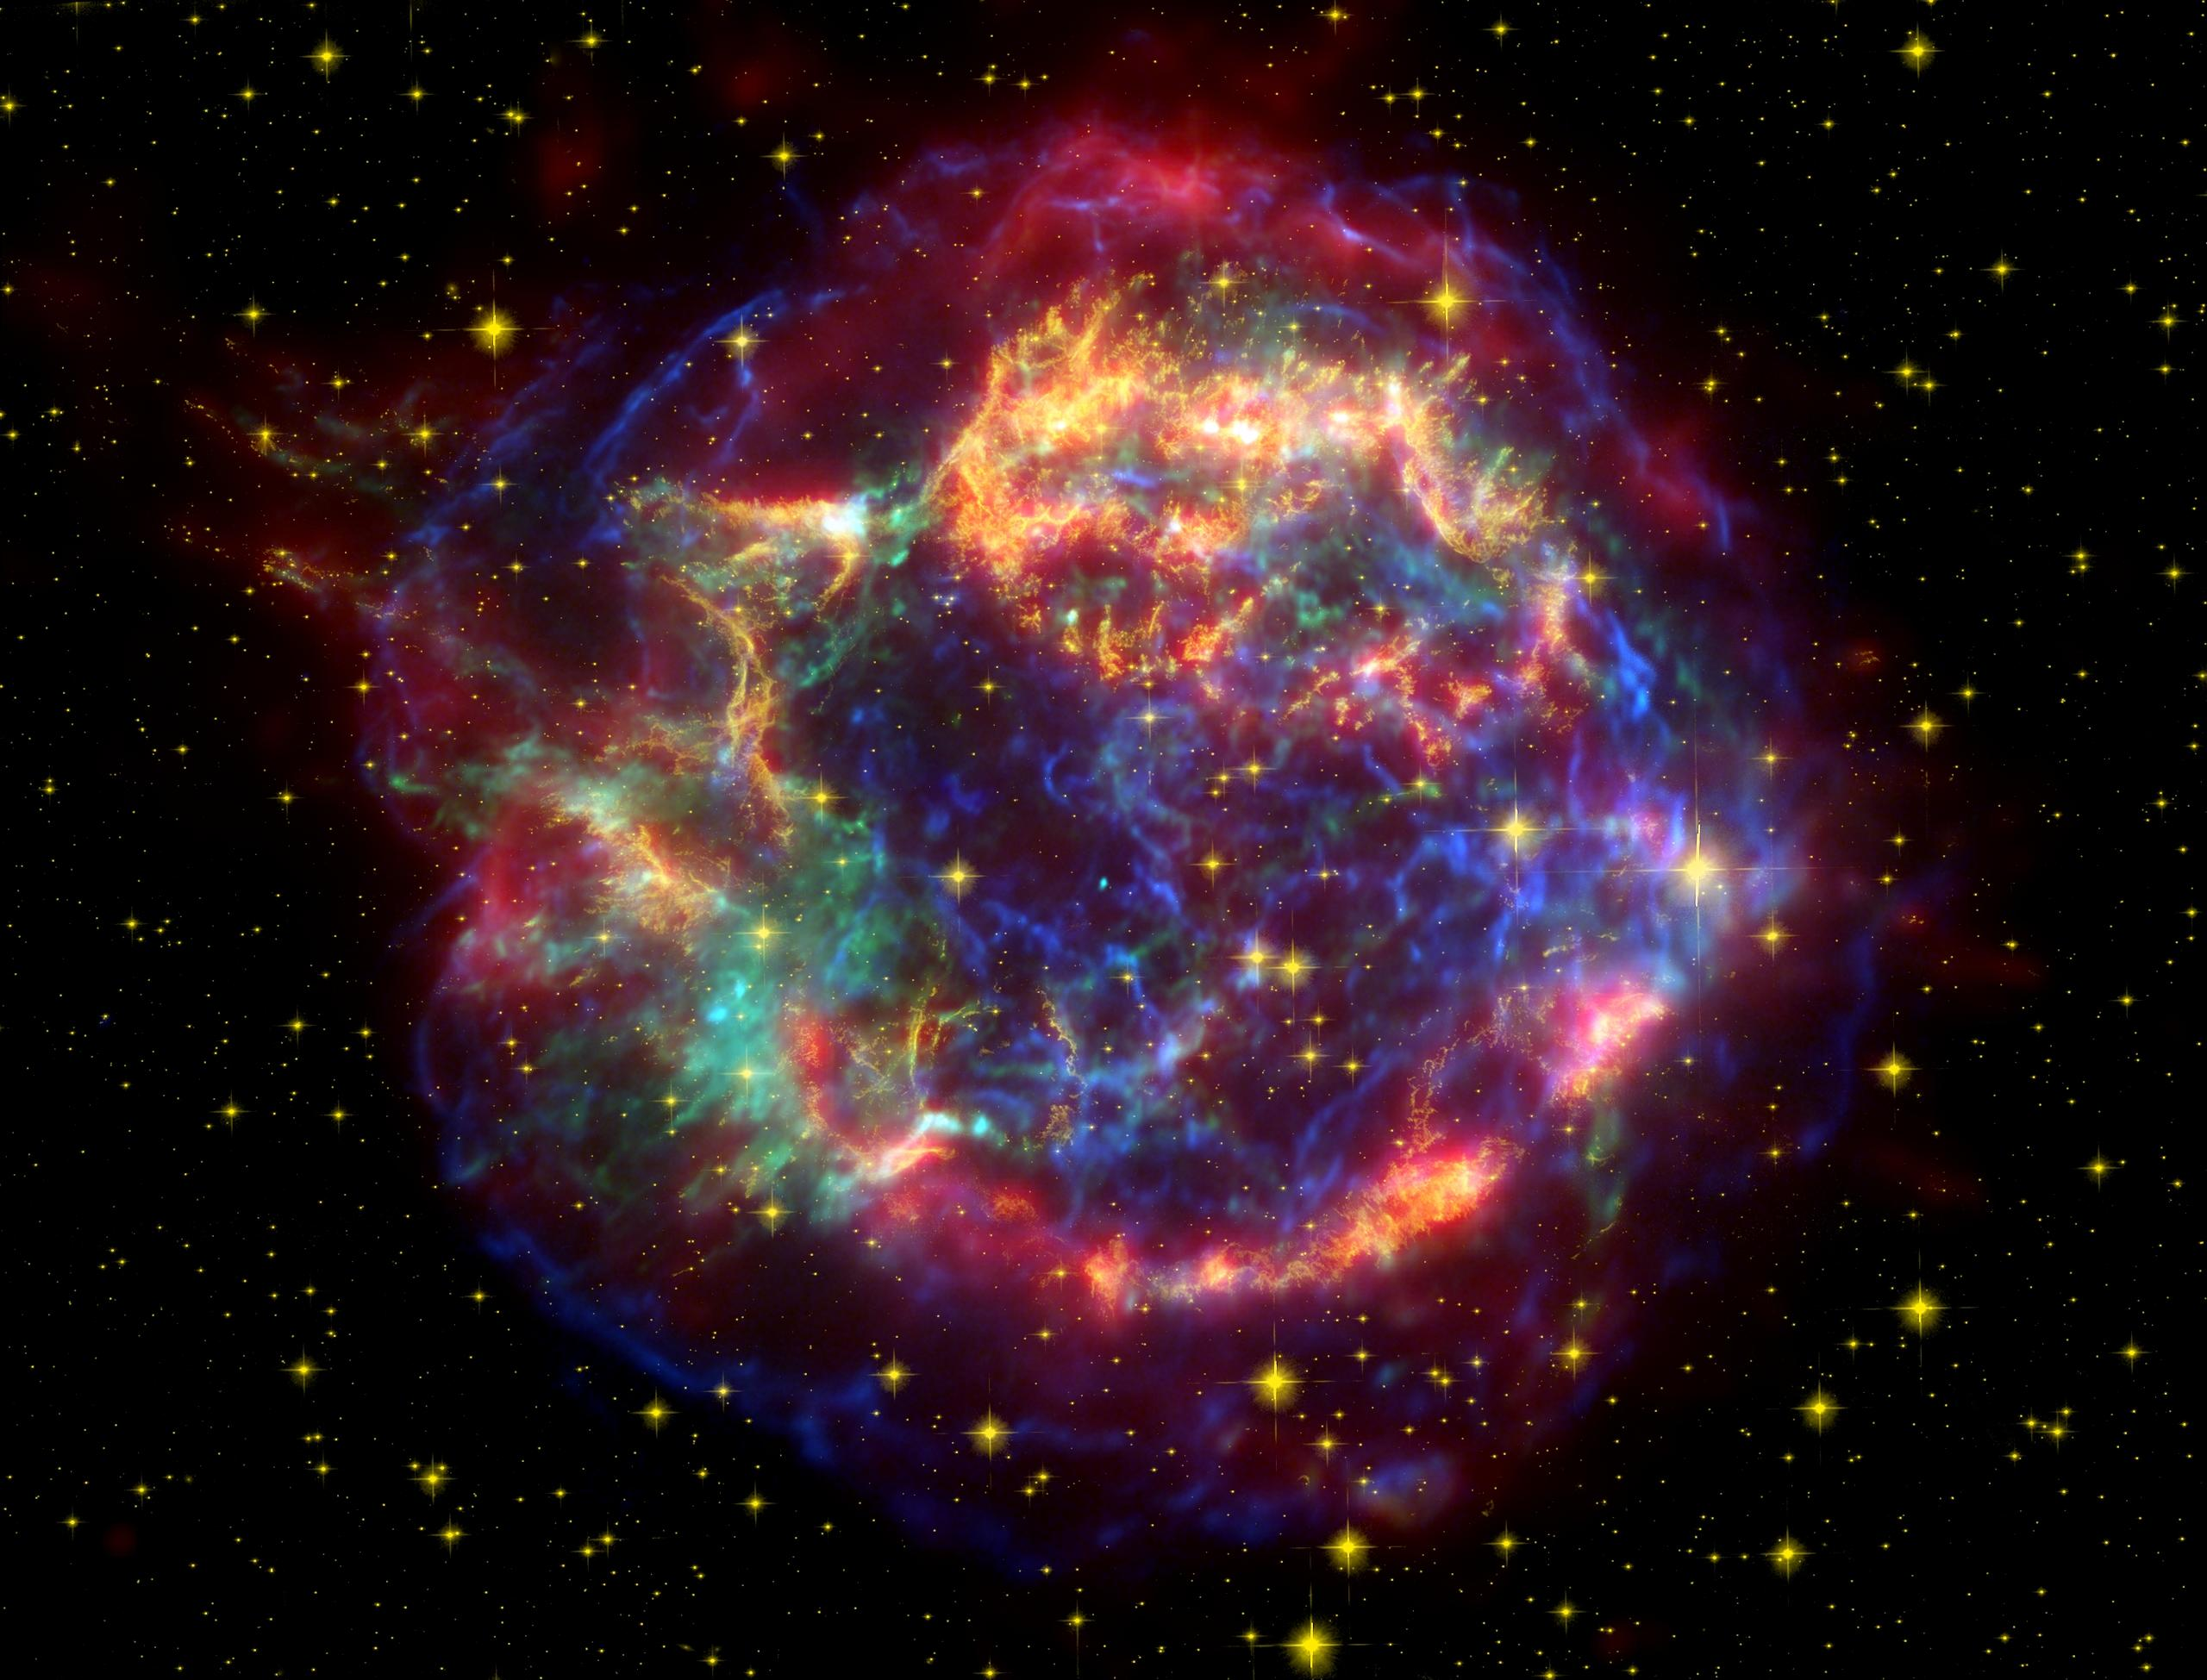
\includegraphics[width=0.7\textwidth]{Cassiopeia_A.jpg}
        \caption{Cassiopeia-A}
        \label{Cassiopeia-A}
    \end{figure}

Una ecuación simple aproxima el radio de la burbuja, $R$, en metros, dada la densidad del gas a través del cual viaja, $N$, en $\atoms/\m^3$, y la energía total, $E$, de la explosión en $\J$:

$$
R(E, N, t) = 2.4 \times 10^8 \left( \frac{E}{N} \right)^{1/5} t^{\,2/5} \; \m.
$$

\vspace{5mm}

\begin{enumerate}
	\item Los astrónomos suelen poder determinar el tamaño de un remanente de supernova y estimar la densidad y la energía, pero desean conocer la edad de la envoltura en expansión. ¿Cuál es la función inversa $t(R, E, N) $ dada la fórmula anterior?

	\item A partir de datos históricos, los astrónomos podrían conocer la edad del remanente de supernova, pero querrían determinar cuánta energía estuvo involucrada en su creación. ¿Cuál es la función inversa $E(R, N, t)$?

	\item El remanente de supernova Cassiopeia-A tiene una edad de unos 500 años y un diámetro de 10 años luz. Si 1 año luz equivale a $9.3 \times 10^{12} \km$, y la densidad media del medio interestelar es $10^6\ \atoms/\m^3$, ¿cuál es la energía involucrada en la explosión de la supernova?
\end{enumerate}
\end{problema}
[7.4.1]
\newpage

\begin{problema}
Los agujeros negros se encuentran entre los objetos más peculiares de nuestro universo. Aunque pueden detectarse a grandes distancias, los futuros viajeros que se atrevan a orbitar uno de ellos experimentarán cambios muy peculiares. Examinemos un pequeño agujero negro con la masa de nuestro Sol. Su radio estará definido por el tamaño de su horizonte, que se encuentra a una distancia del centro del agujero negro de $r = 2.8 \km$.

    \begin{figure}[H]
        \centering
        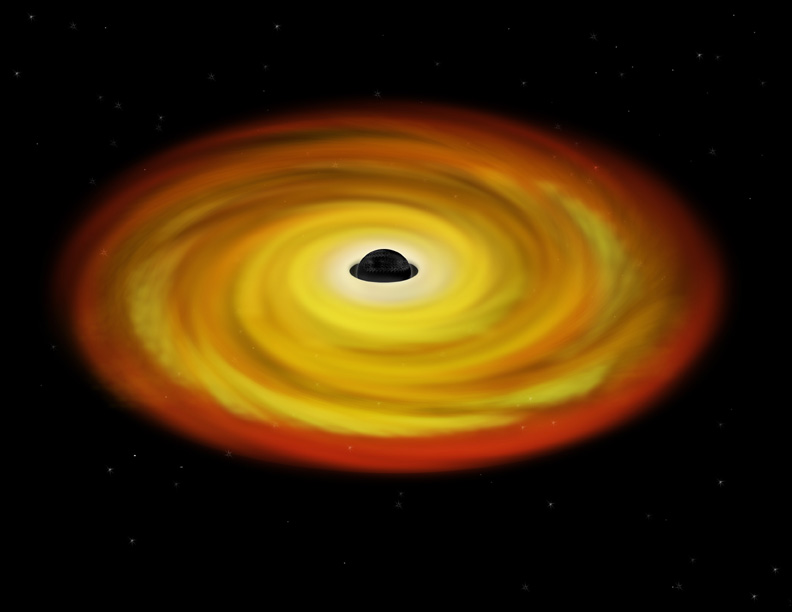
\includegraphics[width=0.7\textwidth]{BlackHoleSpin.jpg}
        \caption{Una representación artística de la materia que fluye hacia un agujero negro en el centro de un disco de acreción.}
        \label{BlackHoleSpin}
    \end{figure}

Un observador distante en la Tierra verá que el reloj llevado por el Viajero comienza a ralentizarse según la fórmula:

$$
T = \frac{t}{\sqrt{1 - \frac{2.8}{r}}}
$$

donde $t$ es el tiempo que pasa en el reloj del Viajero y $T$ es el intervalo de tiempo que un Observador distante percibe.
\begin{enumerate}
	\item El Observador sabe que el reloj del Viajero marca un tic cada segundo, de modo que \( t = 1.0 \). Encuentre la función inversa $r(T)$ que da la distancia del Viajero, $r$, desde el centro del agujero negro en términos del intervalo de tiempo, $T$, medido por el Observador en la Tierra.

	\item El Observador ve cómo el reloj del Viajero se vuelve cada vez más lento. Si el Observador mide los tics a intervalos de $T = 5 \s, \quad 20 \s, \quad \text{y}\quad 60 \s$, ¿a qué distancia del horizonte de eventos ($R = 2.8 \km$) del agujero negro, en metros, se encuentra el Viajero en cada caso?
\end{enumerate}
\end{problema}
[7.4.2]

\newpage
\begin{problema}

La velocidad del sonido, $S$ en $\m/\s$, se puede calcular mediante la fórmula:

$$
S = 108 \sqrt{\frac{T}{m}}
$$

donde $m$ es la masa molecular promedio del gas en $\g/\mol$, y $T$ es la temperatura del gas en $K$.

    \begin{figure}[H]
        \centering
        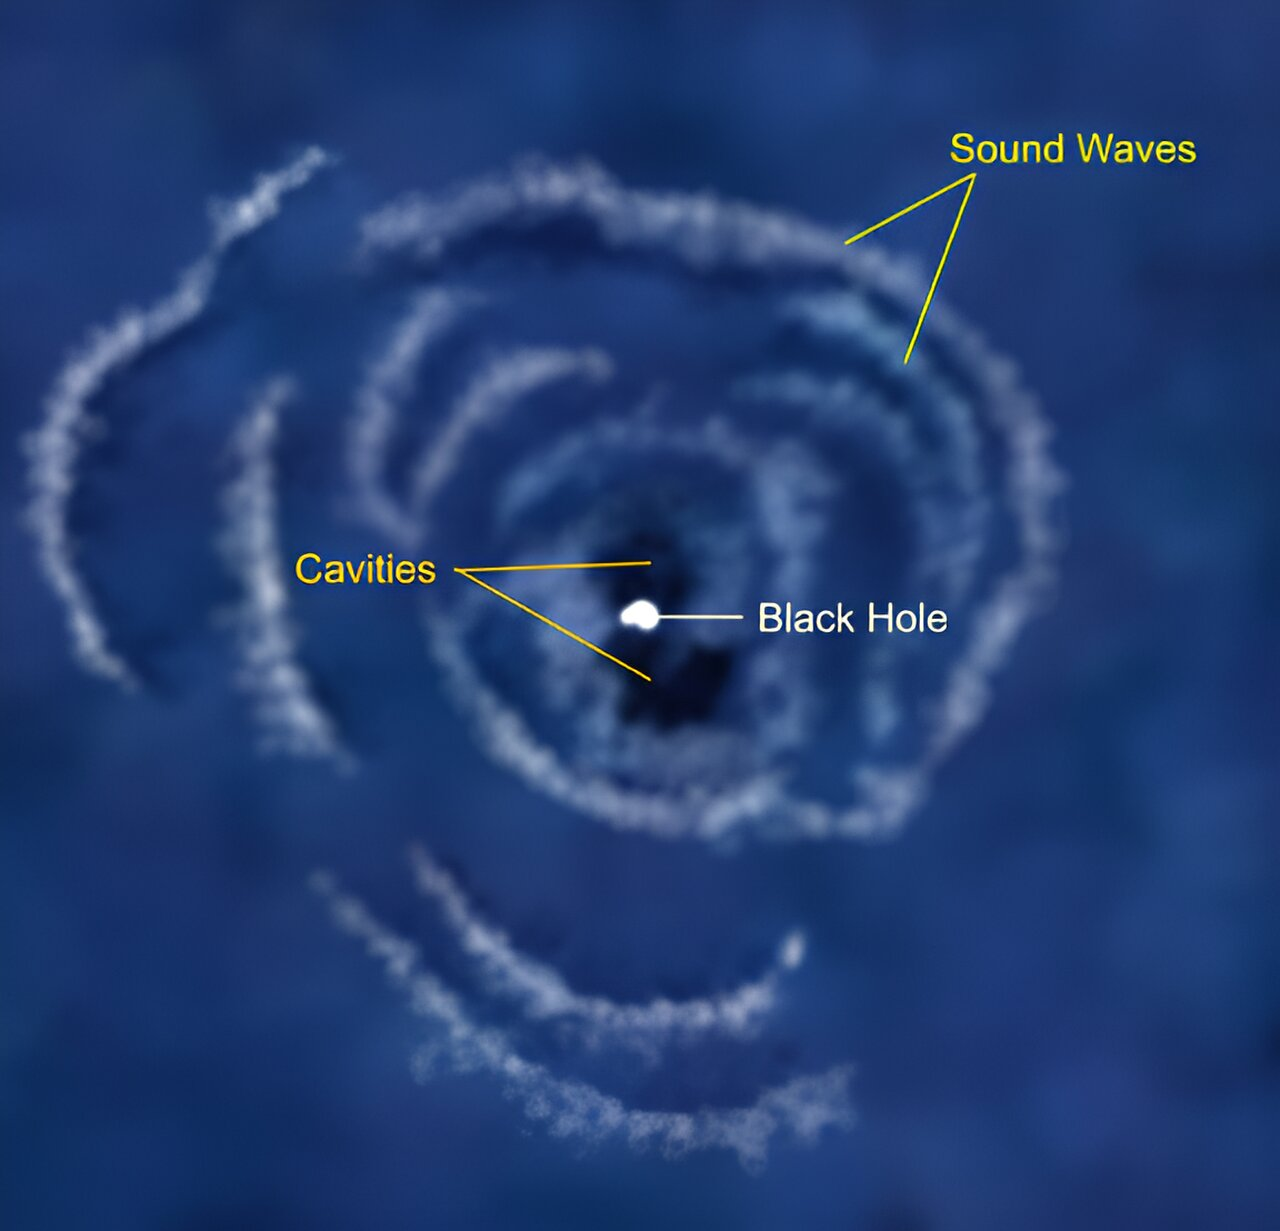
\includegraphics[width=0.7\textwidth]{SoundWaves.jpg}
        \caption{Este esquema, basado en datos del Observatorio Chandra, identifica ondas sonoras que escapan de las cercanías del masivo agujero negro en el centro del cúmulo de galaxias de Perseo. ¡Toma 20 millones de años para que una onda recorra 1 millón de años luz! (Cortesía NASA/Chandra)}
        \label{SoundWaves}
    \end{figure}

\vspace{5mm}
\begin{enumerate}
	\item ¿Cuál es la función inversa que proporciona la temperatura del gas en términos de su velocidad del sonido $T(S)$?

	\item ¿Cuál es la función inversa que proporciona la composición del gas, $m$, en términos de su velocidad del sonido $m(S)$?

	\item A una temperatura de $300 \K$, la velocidad del sonido se mide en $450 \m/\s$. ¿Cuál es la masa molecular promedio inferida del gas?
\end{enumerate}
\end{problema}
[7.4.3]

\cite{algebra2}
\bibliographystyle{plainurl}
\bibliography{bibliografia} % Nombre del .bib

\end{document}